\documentclass[a4paper]{article}

\pdfoutput=1
\usepackage[utf8]{inputenc}
\usepackage[super,sort&compress,comma, square]{natbib}
%\renewcommand{\supercite}[1]{\cite{#1}}

%% Language and font encodings
\usepackage{gensymb}
\usepackage[english]{babel}
\usepackage[T1]{fontenc}
\usepackage{csquotes}
\usepackage{doi}
\usepackage{eurosym}
%% Sets page size and margins
\usepackage[a4paper,top=3cm,bottom=2cm,left=3cm,right=3cm,marginparwidth=1.75cm]{geometry}

% Useful packages
\usepackage{amsmath}
\usepackage{graphicx}
\usepackage{hyperref}
\hypersetup{colorlinks=true, allcolors=blue}
\usepackage{authblk}
\usepackage{multirow}
\usepackage{nomencl}
\usepackage{booktabs}
\usepackage{tabularx}
\usepackage{textcomp}
\usepackage{amsfonts}
\usepackage{outlines} %%same
\usepackage{subfig}
\usepackage[version=4]{mhchem}
\usepackage{siunitx}
\usepackage{bm}
\usepackage[normalem]{ulem} %%temporary, for organization purposes

\date{}
\newcommand{\red}[1]{\textcolor{red}{#1}}
\DeclareSIUnit\angstrom{\text {Å}}
\usepackage[final]{changes}

\interfootnotelinepenalty=10000
% Changed idea title idea from orignal title of
% "Towards a free high quality powder x-ray diffractogram database"
% Name is supposed to be in analogy with Crystallography Open database
% which is the largest freely available database of crystal structures
\title{opXRD: Open Experimental Powder X-ray Diffraction Database}

\author[1,2]{Daniel Hollarek}
\author[1,2]{Henrik Schopmans}
\author[1,2]{Jona Östreicher}
\author[2]{Simon Schweidler}
\author[3]{Adie Alwen}
\author[4]{Mriganka Singh}
\author[4,5]{Tim Kodalle}
\author[6]{Hanlin Hu}
\author[7]{Gregoire Heymans}
\author[8]{Alexander Wieczorek}
\author[10]{Arthur Hardiagon}
\author[11]{Bin Cao}
\author[12, 13]{Maged Abdelsamie}
\author[8]{Siarhei Zhuk}
\author[2]{Ben Breitung}
\author[8]{Sebastian Siol}
\author[9]{Moritz Wolf}
\author[10]{François-Xavier Coudert}
\author[14]{Ruth Schwaiger}
\author[11]{Tong-yi Zhang}
\author[4]{Carolin M. Sutter-Fella}
\author[3]{Andrea M. Hodge}
\author[1,2]{Pascal Friederich}

% I made the affiliations smaller because there's a lot of them
\renewcommand\Affilfont{\small}

\affil[1]{Institute of Theoretical Informatics, Karlsruhe Institute of Technology, 76131 Karlsruhe, Germany}
\affil[2]{Institute of Nanotechnology, Karlsruhe Institute of Technology, 76131 Karlsruhe, Germany}
\affil[3]{Department of Chemical Engineering and Materials Science, University of Southern California, Los Angeles CA 90089, USA}
\affil[4]{Lawrence Berkeley National Laboratory, Molecular Foundry Division, Berkeley 94720 CA, USA}
\affil[5]{Lawrence Berkeley National Laboratory, Advanced Light Source, Berkeley 94720 CA, USA}
\affil[6]{Hoffmann Institute of Advanced Materials, Shenzhen Polytechnic, Shenzhen 518055, China}
\affil[7]{Lawrence Berkeley National Laboratory, Chemical Sciences Division, Berkeley 94720 CA, USA}
\affil[8]{Empa~–~Swiss Federal Laboratories
for Materials Science and Technology, 8600 Dübendorf,
Switzerland}
\affil[9]{Engler-Bunte-Institut \& Institute of Catalysis
Research and Technology, Karlsruhe Institute of Technology, Karlsruhe, Germany}
\affil[10]{Chimie ParisTech, PSL University, CNRS, Institut de Recherche de Chimie Paris, 75005 Paris, France}
\affil[11]{Guangzhou Municipal Key Laboratory of Materials Informatics,  Hong Kong University of
Science and Technology (Guangzhou), Guangzhou 511400, China}
\affil[12]{Material Science and Engineering Department, King Fahd University of Petroleum and Minerals (KFUPM), Dhahran 31261, Saudi Arabia}
\affil[13]{Interdisciplinary Research Center for Intelligent Manufacturing and Robotics, KFUPM, Dhahran 31261, Saudi Arabia}
\affil[14]{Institute of Energy Materials and Devices, Forschungszentrum Juelich GmbH, 52425 Juelich, Germany}
\begin{document}

\maketitle
\begin{abstract}
Powder X-ray diffraction (pXRD) experiments are a cornerstone for materials structure characterization.
Despite its widespread application, the analysis of the diffractograms still presents a significant bottleneck
in high-throughput experimentation that remains to be solved in order to match the increased throughput
of the prior stages of experimentation. In the current landscape of powder X-ray diffraction analysis, machine learning has emerged as a promising research direction to resolve this bottleneck by enabling automated powder diffraction analysis.
A notable difficulty in applying machine learning to this domain is the lack of labeled datasets, i.e.\
diffraction patterns originating from experiment with accompanying structure solutions, which has relegated machine learning
researchers to train on simulated data.
Since these simulations largely fail to accurately reflect the experiment, the performance of models trained
on this simulated data by and large fails to transfer to experiment and provide value in practice.
We aim to remedy this by providing a freely available and easily accessible dataset of partially labeled
powder diffraction data, providing machine learning researchers with a large quantity of real experimental diffractograms collected from a broad range of samples.
We hope that this can guide machine learning research toward more realistic handling of experimental imperfections to enable the improvement of current automated analysis workflows.
\end{abstract}

\newpage
\section{Introduction}\label{sec:Introduction}
% High throughput experimentation
The advent of high-throughput experiments holds the prospect of significantly accelerating the speed of materials discovery\cite{Liu2019}. The synthesis and characterization of novel materials are becoming increasingly efficient and automated, increasing the throughput of samples in experimentation pipelines\cite{MacLeod2019, Ludwig2019, Ozaki2020}. \\

% On Rietveld refinement
After fabricating a new material, a number of analysis techniques can be used to characterize the sample. One method that can be used for phase identification, phase quantification, grain size characterization, and partially to determine the crystal structure of a new material is powder X-ray diffraction. To determine crystal structure from pXRD data, an initial guess is optimized using Rietveld refinement. In this process, an initial crystal structure including unit cell parameters is provided by the operator of the analysis software and fitted to the observed diffractogram in an iterative optimization process based on simulated forward prediction of expected pXRD diffractograms given the current crystal structure\cite{Dinnebier2019, Cano2021}. As Rietveld refinement is a local optimization method, the result of the refinement procedure is only as good as the initial guess it was provided with. \\

% Manual vs (ML) automated Refinement
Manually performing Rietveld refinement is time-consuming and often requires expert knowledge. It is not scalable to the degree required to keep up with advances in throughput and efficiency in other steps of the experimentation pipeline. In a Rietveld refinement process, the operator starts by setting parameters that characterize the background and peak shape of the powder diffraction pattern and determining a crystal structure from which the optimization process can start. The latter is usually done using search-match software, which identifies crystal structures with similar powder diffraction patterns from a database of crystal structures with accompanying powder diffraction patterns. However, attempting to refine all crystal structure parameters at once, starting from this initial structure, is known to lead to unphysical results. What makes the refinement process time-consuming and difficult is finding the correct order in which to refine the crystal structure parameters\cite{Ozaki2020}.  Additionally, if the fit develops into an unphysical set of parameters in this iterative determination of parameters, the operator must intervene to backtrack to the last step. \\

Commonly used databases for obtaining a match include the Powder Diffraction File\cite{GatesRector2019}, the Inorganic Crystal Structure Database \cite{Belsky2002}, and the Crystallography Open Database \cite{Grazulis2009}. An initial guess obtained from such a database is by no means guaranteed to lead to an accurate structure solution, even if it is iteratively revised, either manually or using blackbox optimization\cite{Ozaki2020}. Especially for novel observed structure types, simply matching to a database of known structures will not yield good results. Therefore, more complex crystal structure solution approaches need to be applied to find suitable crystal structure guesses. \\


Machine learning has the potential to speed up the manual analysis of powder diffractograms and keep pace with an automated high-throughput experimentation environment\cite{Agrawal2019, Surdu2023}.
Models can be trained to predict crystal structure information directly given a diffractogram, or models can be used to automate the conventional workflow of finding an initial guess \cite{Surdu2023} and running ML-automated Rietveld refinement \cite{Feng2019}.
So far, however, due to an absence of labeled datasets with experimental diffractograms\cite{Wang2020}, machine learning in this domain has largely relied on diffractograms simulated from known structures\cite{Park2017, Lee2023} or, most recently, from generated synthetic crystals\cite{Schopmans2023}. \\

% Predicting structure information with machine learning
Models trained on datasets with simulated diffractograms have already shown very strong performance in predicting lattice parameters\cite{Dong2021, Chitturi2021, Habershon2004, zhang2024crystallographic}, spacegroup \cite{Schopmans2023, Oviedo2018, Park2017, Vecsei2018, Zaloga2020, Suzuki2020, Chakraborty2021,zhang2024crystallographic}, and crystallite size \cite{Dong2021, Chakraborty2021} from simulated diffractograms.
However, the performance substantially drops off when these models are applied to data originating from experiments \cite{Schopmans2023,zhang2024crystallographic}[cite 2-3 papers, incl. ours].
The patterns observed in experiments exhibit imperfections that do not appear when simulating the X-ray diffraction pattern of a powder sample under ideal conditions. The physical effects underlying these imperfections need to be modeled accurately in order to be able to transfer models trained on simulated data to experimental patterns. Most approaches currently model these imperfections as a simple signal based on a heuristic functional form added to the simulated diffractograms.

At the moment, the number of openly available datasets for experimental powder data is very limited. The main sources for experimental patterns are XXX, YYY, and ZZZ. Further commercial datasets such as KKK and LLL exist, but license fees and restrictions in their use to train publishable models or even publish the training data limit their usability. Collecting a labeled dataset of raw experimental powder X-ray diffraction data of sufficient size to directly train a model that predicts crystal structure information is likely out of reach. The most advanced ML models currently are trained on approximately $10^7 - 10^8$ simulated diffractograms, which is - to the best of our knowledge - three orders of magnitude larger than the largest currently curated experimental dataset (PDF-5+ with approximately 20,000 experimental patterns) and even x orders of magnitude larger than the number of unlabeled diffractograms in the opXRD dataset we present here. \\

However, even small labeled and also unlabeled experimental diffractograms hold significant value in practice. First of all, labeled data can be used to better test and benchmark existing and new automated analysis approaches, which yields a better comparison than when using the very limited currently available datasets, such as the commonly used RRUFF mineral dataset\cite{Armbruster2015}. \\

Furthermore, even completely unlabeled data can enable machine learning researchers to evaluate how closely their simulations represent experimental data, identify what features are missing, and modify their simulation algorithms accordingly to arrive at a simulation that mirrors how data appears in reality. In this way, one can bring the simulated patterns closer to those observed in experiments by more accurately modeling the scattering process.
Improving the simulation of data involves accounting for more of the physical effects that influence the scattering process such as preferred grain orientation, variations in grain size, crystal defects, the impact of temperature on the scattering process, internal stress, and X-ray-induced fluorescence\cite{cao2024simxrd, Waseda2011, Pecharsky2023}.  Additionally, it should be considered that varying experimental setups can produce distinct powder diffraction patterns on the same sample. Features that may vary between experimental setups and influence the recorded pattern include the shape of diffraction peaks, the wavelength and polarization of the employed X-ray source, and the detector geometry
\cite{Waseda2011, Pecharsky2023}. Some experimental setups may also exhibit imperfections such as displacement of the sample from its intended position leading to the recorded scattering angles being slightly erroneous \cite{hulbert2023} or background events originating from instrument noise or X-rays scattering off equipment onto the screen.\\

Additionally, some of the observed imperfections, such as background and noise, can be accounted for using transfer learning approaches. In transfer learning the objective is to transfer the capabilities of a model learned on a source domain in which labeled data is abundant to a target domain in which labeled data is sparse\cite{Zhuang2021}. In this context, the source domain is simulated powder diffraction patterns and the target domain is experimental powder diffraction patterns. Many approaches to transfer learning have been proposed, particularly in the domain of image classification \cite{Gatys2016, Ganin2015}. These existing techniques could potentially be adapted to facilitate transfer learning in the context of pXRD patterns.

In this publication, we provide a new open powder X-ray diffraction (opXRD) dataset that collects a broad range of patterns from experiments, exceeding the currently available amount of openly accessible experimental patterns by XX.
Our opXRD dataset has been curated by collecting the accumulated powder data from multiple large research groups and institutions with high-throughput XRD facilities. It contains pXRD patterns from single and multiphase materials from a wide variety of materials classes, including XXX, YYY, and ZZZ. Details about the experiments of contributing research groups are discussed in this paper, along with a detailed description of how to contribute further data and how to use the data. \\

\begin{figure*}[!htb]
    \centering
    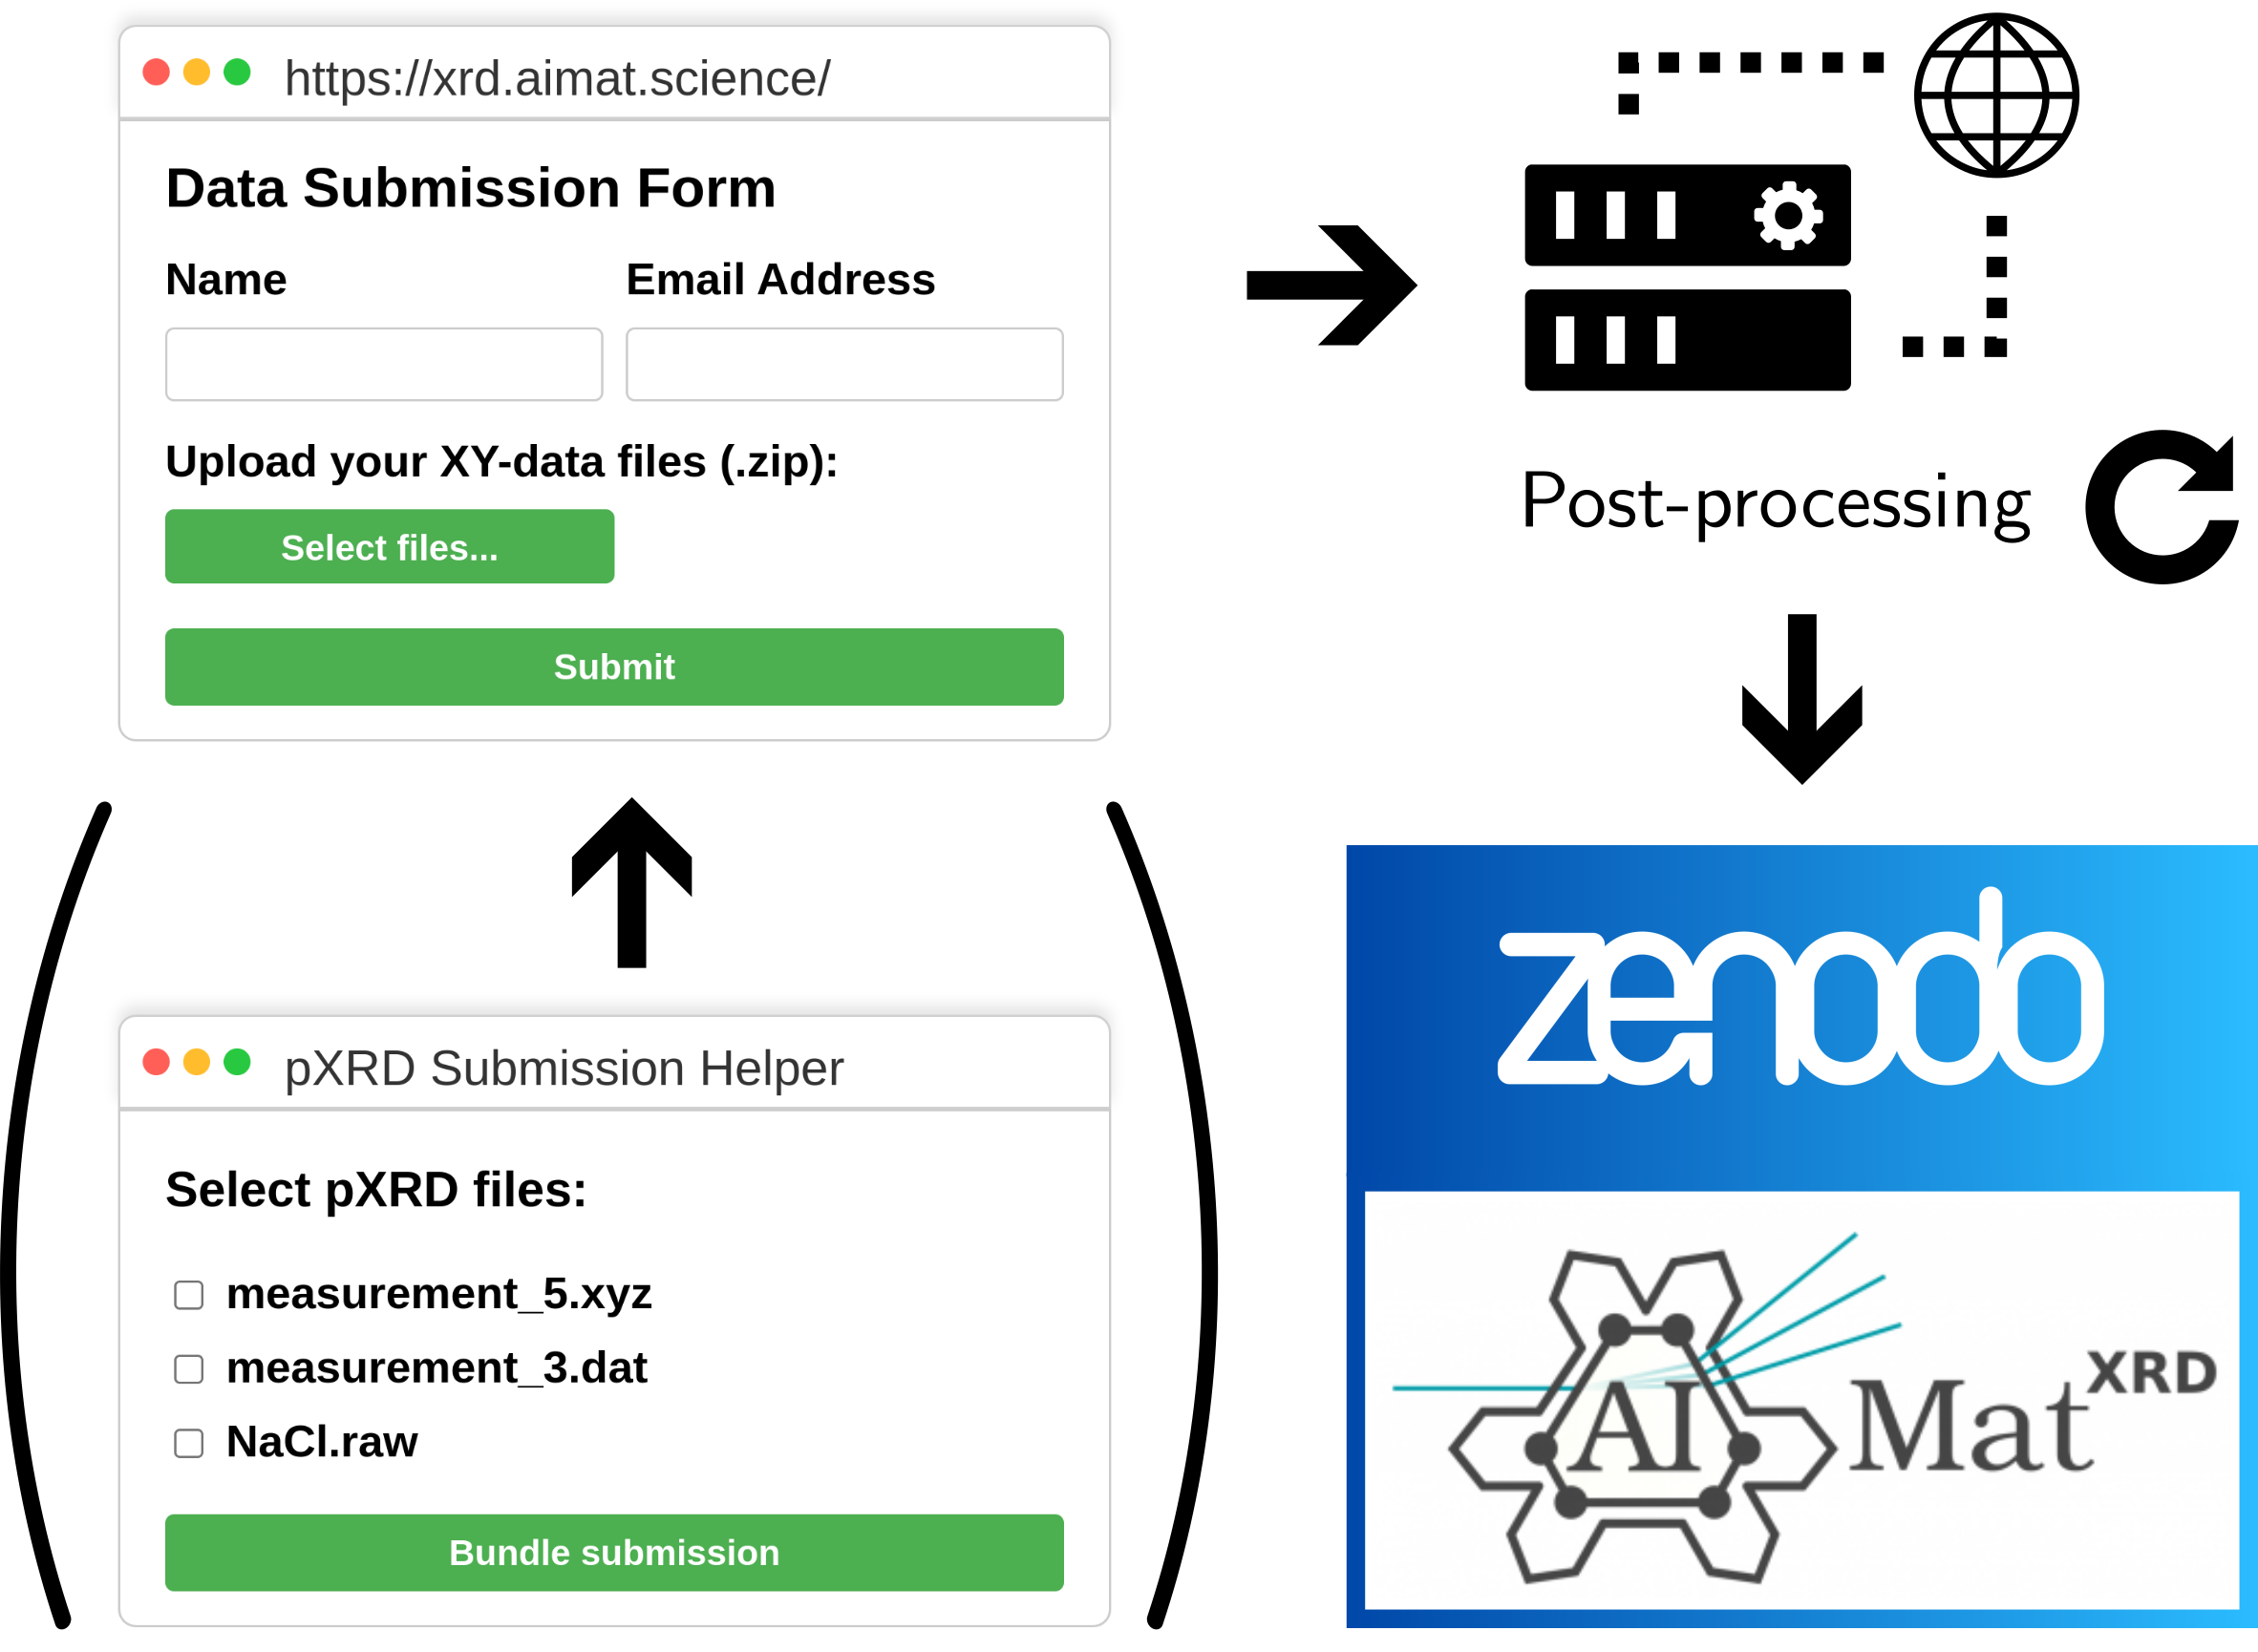
\includegraphics[width=\linewidth]{figures/overview2.png}
    \caption{Overview of the data collection pipeline. Datasets are submitted using an online submission form or our submission helper software. After post-processing and data homogenization, we create a Zenodo entry for each user submission and subsequently include the submission in the opXRD database.}
    \label{fig:overview}
\end{figure*}

% How to contribute? This aspect deserves a separate paragraph
The opXRD database is planned as a growing, community-driven initiative. The dataset we present here is the first version, but we hope to further increase the dataset size through active engagement with the pXRD community. Our primary objective is to minimize the effort and thus the barrier to contributing experimental data to the opXRD database. Thus, we developed a program that helps to find and share data from e.g. pXRD lab computers. In detail, users can select their most common pXRD file types, the program lists all files of that type, and users can select or deselect certain folders or files for sharing. Selected contributions will be uploaded to opXRD, processed to a common file format, and - if wanted - published on Zenodo on behalf of the contributors, before becoming part of the opXRD database. If labels are available, they can be shared with opXRD as well. Further details can be found on the opXRD website (Figure~\ref{fig:overview}). \\

As argued by Aranda and Kroon-Batenburg \textit{et al}.\cite{Aranda2018, Kroon-Batenburg2024}, sharing raw powder diffraction data is not only in the interest of furthering machine learning research but is also in line with open science principles. It furthers the ability of other researchers to reproduce published work and in turn, adds to the credibility of the publisher of the data. Considering our streamlined submission and post-processing framework, a publication of powder diffraction data through the opXRD database is a simple way of realizing these principles. Compared to uploading the data to Zenodo it also has the added benefit that the data is contributed towards a large, homogenous dataset with a standardized interface. This makes the data more easily accessible to other researchers and provides more value to researchers seeking great quantities of data compared to an isolated submission on Zenodo. \\


The broad range of available experimental samples contained in the opXRD v1.0 database makes it possible to apply state-of-the-art ML approaches to the domain of powder XRD analysis. We hope that this can drive ML research in this field towards more advanced automated analysis workflows that can accelerate material science research through ready application in high-throughput experimentation pipelines.

\*section{Existing datasets}
% Datset listing (List written on 20.06.24)
% Lists of Crystallographic databases; Our list contains all of the databases given in the lists linked below
% - IUCR: "Crystallographic databases and related resources" (https://www.iucr.org/resources/data/databases)
% - Bruno et al. (2017): "Crystallography and Databases" (https://datascience.codata.org/articles/10.5334/dsj-2017-038)
% - University of Virginia "Crystallographic data" (https://guides.lib.virginia.edu/c.php?g=514782&p=3568808)

% [X] 1 PDF5+ (https://www.icdd.com/,https://www.icdd.com/pdf-5/) -> 19000 structures with pXRD patterns | I checked with their support
    % (1.1): ICDD Powders
    % (1.2): FIZ ICSD (https://icsd.products.fiz-karlsruhe.de/)
    % (1.3): NIST ICSD https://icsd.nist.gov/
    % (1.4): Linus Pauling File (https://paulingfile.com/index.php?p=about%20us)
    % (1.5): ICDD Single Crystal data
% [x]: 2 COD (https://www.crystallography.net/cod/) -> ~ 1000 structures with real pXRD patterns | These patterns were extracted by PSL university
% [x]: 3 RRUFF (American Mineralogist Crystal Structure Database) -> ~ 1000 structures with real pXRD patterns | We downloaded the entire dataset and discarded single crystal data
% [x]: 4 CCDC (https://www.ccdc.cam.ac.uk/) -> No exp pXRD | There is only mention of simulated powder diffraction data. Of 20 sampled cifs none contained powder diffraction data
% [x]: 5 The Material Project (https://legacy.materialsproject.org/) -> No exp pXRD | The only mention of available X-ray diffraction data is of simulated data
% [x]: 6 Crystal Lattice Structures (https://www.atomic-scale-physics.de/lattice/) -> No exp pXRD | Their entries provide no X-ray diffraction data, and also most links appear broken
% [x]: 7 Crystallographic and Crystallochemical Database for Minerals and their Structural Analogues (https://database.iem.ac.ru/mincryst/) -> No exp pXRD | The given powder diffraction data is simulated (see: Powder X-ray Diffraction Standards (CPDS) @ https://database.iem.ac.ru/mincryst/descript.htm)
% [x]: 8 Mineralogy Database (https://webmineral.com/) -> No exp pXRD | I checked with the author of the site
% [x]: 9 IUCr Raw data letters (https://iucrdata.iucr.org/) -> No exp pXRD | There are only two raw data letters, both of them single crystal data
% [x]: 10 Bilbao Crystallographic server  (https://www.cryst.ehu.eus/bincstrdb/search/) No exp pXRD | Of 20 sampled CIFs out of 256 entries none contained pXRD data
% [x]: 11 PowBase (http://www.cristal.org/powbase/index.html) -> 169 real pXRD patterns some of which have at least partial labels; The described submission process and the lack of crystal structures indicate that the patterns are not simulated
% [x]: 12 Athena (https://athena.unige.ch/athena/mineral/mineral.html) -> No exp pXRD | No mention of diffraction data anywhere
% [x]: 13 Protein database (https://www.rcsb.org/) / NAKB (https://www.nakb.org/) / BMCD ((http://bmcd.ibbr.umd.edu/)  -> Little to no exp pXRD | Of the 230k structures only 21 showed up when searching experimental method = Powder diffraction
% [x]: 14 Crystal Met (https://cds.dl.ac.uk/cds/datasets/crys/mdf/llmdf.html) -> No exp pXRD | The only mention of diffraction data is simulated data
% [x]: 15 Pearson's Crystal data (https://www.crystalimpact.com/pcd/) -> 21700 experimental powder diffraction patterns (As per https://www.crystalimpact.com/pcd/) | The Pearson's crystal data evolved from the Linus Pauling File which is a data source of the PDF, so there may be significant overlap in these patterns
% [x]: 16 Zenodo powder diffraction data (https://zenodo.org/search?q=powder%20diffraction&l=list&p=1&s=10&sort=bestmatch) -> Some pXRD data but hard to quantify, probably <= 4000 patterns most of which are unlabeled | 1600 datasets matching "powder diffraction". From probing among the first 100 matches I estimate only about 1 in 10 contain powder diffraction patterns. The probed datasets that did contain powder diffraction data only contained <= 30 patterns and only one of them came with corresponding crystal structures

%TODO: Summarize the existing datasets shortly, including number of entries, etc.

\pagebreak

\subsubsection*{Existing experimental powder diffraction datasets}
To contextualize opXRD within the current environment of experimental powder diffraction data, the following list provides an overview of the largest crystal structure databases that include powder diffraction data.  \\

\textbf{Powder Diffraction File:}\footnote{More information on the Powder Diffraction File can be found under \url{https://www.icdd.com/pdf-5/}.} The Powder Diffraction File (PDF), published and maintained by the International Center for Diffraction Data (ICDD), is a large collection of materials with accompanying powder diffraction data. Its latest release as of November 2024, the PDF5+, contains over a million materials with accompanying powder diffraction data. However, most of these powder diffraction patterns are simulated. After inquiring with the ICDD in April 2024 we were told that only 19000 of the powder diffraction patterns in the PDF5+ stemmed from experiments. \footnote{We reached out to the contact address given on their website, info@icdd.com.} Still, this makes the PDF5+, to the best of our knowledge, the largest collection of experimental powder diffraction data available to researchers. As of November 2024, the PDF5+ is available to researchers through a purchase starting at a price point of \$6,265.00.\\

\textbf{Crystallography Open Database:}\footnote{More information on the crystallography open database can be found under \url{https://www.crystallography.net/cod/}.} The Crystallography Open Database (COD)\cite{Graulis2009cod} is an open-access collection of crystal structures. It provides over 500.000 crystal structures in the form of .cif files. Of these files, 1063 contained the experimental powder diffraction data that was used to determine the underlying crystal structures of the investigated samples. \\

\textbf{RRUFF}: The RRUFF Mineral Database \cite{Armbruster2015} provides detailed information on minerals, including their chemical compositions, crystallography, and spectroscopic data. Managed by the University of Arizona, it was created to serve as a public repository for mineral identification and research. It contains \num{908} distinct structures with experimental x-ray diffraction patterns. \\

\textbf{PowBase}: 

\textbf{Pearson's Crystal data}:

Some major crystal structure databases, such as the ICSD, do not appear in the above list, as they do not include powder diffraction data. This is because most structure solutions are achieved through single-crystal diffraction rather than powder diffraction.
 


\*section{Machine learning for pXRD}
\paragraph{ML for pXRD} Several approaches have applied machine learning methods to classification and regression tasks for powder diffractograms.

TODO: We need a short literature review here; needs to also cover papers published after our previous paper!

TODO: briefly discuss here that there are expert models for specific classes of materials which give more information, and more generic models like ours which currently only gives you the space group and not much more; especially focus on how experimental conditions (background, noise, ... is modeled)
Phase Labeling and Lattice Refinement: https://arxiv.org/abs/2308.07897


TODO: briefly discuss papers about multiphase classification and remixing of diffraction patterns
Physically-informed Graph-based DRNet (PG-DRNet): https://ieeexplore.ieee.org/abstract/document/10459774/
https://www.nature.com/articles/s42256-021-00384-1
non-negative matrix factorization: https://ojs.aaai.org/aimagazine/index.php/aimagazine/article/view/2785

TODO: discuss in more detail why domain randomization as we did in the last paper so far failed for background and noise, and thus why we need background and noise statistics from experiment to enhance simulated datasets and transfer them to the experimental data distribution.

\section{opXRD database}\label{sec:our_dataset}
\begin{figure*}[!ht]
    \centering
    \missingfigure{} 
    \caption{Statistics, histograms, etc. of our dataset.}
    \label{fig:statistics}
\end{figure*}

In collaboration with several other institutions we have collected a dataset of diffractograms stemming from experiments, some of them labeled with corresponding structural information. The following texts detail the contribution of each research group. Most data was collected using \ce{Cu} radiaton sources which have a  $K_{\alpha1}$ wavelength of $\lambda=1.54056\text{\AA}$ and a $K_{\alpha2}$ wavelength of $\lambda=1.54439\text{\AA}$.

%% Paragraph by FX Coudert and Arthur Hardiagon
\subsubsection*{Chimie Paris Tech, PSL University}

We extracted experimental pXRD data from the Crystallography Open Database (COD)\cite{Grazulis2009, Vaitkus2023}. The COD is, to our knowledge, the largest open-access collection of experimental crystal structures of organic, inorganic, and metal-organic compounds and minerals, containing more than 500,000 entries. \footnote{Available online at \url{https://www.crystallography.net/cod/}.} The data in the COD is placed in the public domain and licensed under the CC0 License. Of the entire COD database 5432 structures contained at least one tag from the {CIF\_POW} dictionary, i.e., a tag relating to powder diffraction studies. These 5432 structures only account for 1\% of the total COD database, but this is to be expected since most crystal structures are resolved from single-crystal diffraction. Of these 5432 files, most contained only metadata related to the powder diffraction experiment, but did not include the raw data of the pattern itself. We could extract raw experimental pXRD patterns from 1063 files in total, after curation of a small number of files with clearly invalid data. \\

The pXRD data from the COD database are of high quality, with a median resolution of $\Delta(2\theta) = 0.013\degree$ and an average number of 9190 points measured per pattern. They span a wide chemical space, including organic, inorganic, and hybrid structures, including 75 different elements of the periodic table.

%% Paragraph by Ben Breitung
\subsubsection*{Institute of Nanotechnology, KIT}

A major part of the research focused on high-entropy materials, which involved incorporating many different elements into single-phase structures, leading to peak shifts or phase separations. Most of those multi-component complex materials appeared in various structures, including rock-salt, spinel, fluorite, perovskite, and delafossite. The samples were almost always prepared in powder form; therefore, powder XRD was performed on samples with adjusted height. The samples were prepared using various synthesis techniques, mostly solid-state or wet chemical syntheses, to obtain the desired structures. Consequently, particle size and crystallinity varied significantly. The sample set also includes samples that were not successfully measured or where phases could not be identified. \\

The X-ray diffraction data were collected on a Bruker D8 Advance using a Cu radiation source  The samples were initially recorded for various research projects over the last ten years and were measured with different step sizes, times per step, and over different angle ranges, but all using \ce{Cu} $K_\alpha$ radiation. The samples mostly contained transition metal oxides, sulfides, and fluorides. To improve statistics, the samples were rotated during the entire measurement. Some air-sensitive samples were measured using a transparent polymer dome for protection. This dome led to increased background noise over the first $20\degree$ and slightly decreased pattern resolution. \\ 


% Paragraph by Moritz Wolf 
\subsubsection*{Institute of Catalysis Research and Technology, KIT}

A variety of samples were analyzed including commercial catalysts, bulk reference materials, porous metal oxide particles, and nanoparticles. The latter were synthesized via the surfactant-free benzyl alcohol route \cite{Wolf2019, Wolf2018}. The cobalt oxide (\ce{CoO} or \ce{Co3O4}) and cerium oxide (\ce{CeO2}) nanoparticles were in the size range of $4-16 \ \si{nm}$ according to the Scherrer equation. A series of porous \ce{Al2O3} materials, which were prepared by calcination of boehmite (\ce{AlOOH}) at various temperatures, represents crystalline samples with limited long-range structure and various contributions of \ce{Al2O3} polymorphs.\\

X-ray diffraction (XRD) was conducted with an X’Pert Pro MPD (Panalytical) in Bragg-Brentano geometry using a \ce{Cu} X-ray source. The patterns were acquired in the $2\theta$ range of $5-80\degree$ with a step size of $0.016711\degree$ or $0.033420\degree$ and a total acquisition time of 40 to 120 min. \\

% Paragraph by Adie Alwen and Andrea Hodge
\subsubsection*{Department of Chemical Engineering and Materials Science, USC}

Combinatorial \ce{CuNi} and \ce{CuAl} samples were synthesized at the University of Southern California (USC) via magnetron co-sputtering from \ce{Cu} (99.999\%) and \ce{Ni} (99.995\%) or \ce{Al} (99.999\%) targets (Plasmaterials) onto stationary $10 \si{cm}$ \ce{Si} (100) substrates yielding 169 unique $5 \times 5 \ \si{mm}$ squares per wafer. These alloys were selected to study compositional effects on stacking fault and growth twin boundary formation in sputtered materials \cite{2024AcMat.27019839A,alwen2024combinatorial}. XRD spectra were collected using a Malvern Panalytical Empyrean X-ray diffractometer at the Forschungszentrum Julich (FZJ) Institute for Energy and Climate Research, Structure and Function of Materials (IEK-2), which enabled automated XRD characterization due to its programmable XY stage and laser sensor for Z height correction. XRD analysis was used to link changes in defect formation in the sputtered films with varied phases and crystal structures. Each composition was characterized using \ce{Cu} $K_\alpha$ X-rays that were collimated to probe an area of $4 \times 4 \ \si{mm}$ using a step size of $0.026\degree$ and scan duration of $0.3$ seconds per step over a 2 range from $30\degree - 110\degree$. Measurement parameters were chosen to resolve at least six or more points above the full-width half maximum of each XRD peak.

% Paragraph by Tim Kodalle
\subsubsection*{Lawrence Berkeley National Lab}

Data collection was performed in situ during thin-film deposition using a custom-made spin-coating and annealing stage. One dataset was collected from spin-coating triple cation metal-halide perovskite precursor solutions with the composition 
\ce{Cs}$_{0.05}$(MA$_{0.23}$FA$_{0.77}$)\ce{Pb}$_{1.1}$(\ce{I}$_{0.77}$\ce{Br}$_{0.23}$)$_{3}$ (MA = Methylammonium, FA = Formamidinium) onto various substrates, including glass (amorphous), $\ce{GaAs}$ wafers (single crystalline) as well as stacks of glass/ITO, $\ce{GaAs}$/$\ce{Mo}$/$\ce{Cu}$($\ce{In}$,$\ce{Ga}$)$\ce{Se2}$/$\ce{CdS}$/$\ce{ZnO}$, and glass/$\ce{Mo}$/$\ce{Cu}$($\ce{In}$,$\ce{Ga}$)$\ce{Se2}$/$\ce{CdS}$/$\ce{ZnO}$ (glass/CIGS). Some of the substrates were additionally covered with a self-assembling monolayer of MeO-2PACz. The $\ce{GaAs}$ substrates were prepared by Dr. Jiro Nishinaga from the National Institute of Advanced Industrial Science and Technology (AIST) in Japan and the glass/CIGS substrates by Dr. Christian Kaufmann and his team at Helmholtz-Zentrum Berlin (HZB) in Germany. \\

A second dataset was collected from spin-coating metal-halide perovskite precursor solutions with varying compositions of \ce{MAPb(I_{1-x}Br_x)3} (where MA = Methylammonium and x = 0, 0.33, 0.5, 0.67, 1) spin-coated onto glass substrates. The substrates were preheated to different temperatures ($30\degree $C, $50\degree $C, $70\degree $C, and $90\degree $C), and the spin-coating process was performed at a constant temperature on the preheated substrates. For both datasets, diffraction data were continuously measured during spin-coating, chemical induction of crystallization, and annealing of the samples (at $100\degree$C and $110\degree$C respectively) with a frequency of about $0.56 
 \ 1/\si{s}$ and $0.54 \ 1/\si{s}$. Each in situ measurement consisted of about 500 to 1000 individual diffractograms. Depending on the substrate, each series of diffractograms shows an evolution from substrate only to a combination of polycrystalline perovskite, $\ce{PbI2}$ and substrate via several intermediate phases. \\

Experimental XRD data were collected at beamline 12.3.2 of the Advanced Light Source, the synchrotron at Lawrence Berkeley National Laboratory. The data were collected using a photon energy of 10 $\si{keV}$ ($\lambda = 1.23984 \text{\AA}$), selected using a Si(111) monochromator. Measurements were taken in grazing incidence geometry, i.e. using a beam incidence angle of $1\degree$ Two-dimensional diffraction images were recorded using a Dectris Pilatus 1M area detector at an angle between $34\degree$ and $36\degree$ with a sample-to-detector distance of roughly $190 \ \si{mm}$. The two-dimensional data were calibrated using an Al$_{2}$O$_{3}$ calibration standard and integrated along the azimuthal angle. \\


% Paragraph by Bin Cao and Tong-yi Zhang
\subsubsection*{Guangzhou Municipal Key Laboratory of Materials Informatics, HKUST}

In the past two years, we established a small-scale experimental PXRD database called the X-Ray Phase Identification Public Experimental Dataset. The data in XRed is generated in our lab using instruments such as the Empyrean 3.0, Aeris, and Bruker D8 Advance diffractometers under Cu targets. Hundreds of PXRD patterns have been refined, labeled with CIF files, and organized by elemental systems. The dataset includes original experimental files across single-phase to five-phase mixtures. This project is progressing toward integration with the comprehensive opXRD database to establish a large-scale, long-term experimental resource. 

In the past two years, we established a small-scale experimental pXRD database called the X-Ray Phase Identification Public Experimental Dataset (XRed). \footnote{XRed can be found on GitHub at \url{https://github.com/WPEM/XRED}.} The data in XRed is generated in our lab using instruments such as the Empyrean 3.0, Aeris, and Bruker D8 Advance diffractometers using \ce{Cu} X-ray sources. Hundreds of pXRD patterns have been refined, labeled with CIF files, and organized by elemental systems. The dataset includes original experimental files across single-phase to five-phase mixtures. This project is progressing toward integration with the comprehensive opXRD database to establish a large-scale, long-term experimental resource. 

% Paragraph by Alexander Wieczorek and Sebastiann Siol
\subsubsection*{Laboratory for Surface Science and Coating Technologies, Empa}

Each combinatorial Zn–V–N library was synthesized using radio-frequency co-sputtering of Zn and V in a mixed Ar and \ce{N2} plasma. An orthogonal deposition temperature and composition gradient was created, resulting in a deposition temperature of $220\degree$C for samples 1~–~9 and $114\degree$C for samples 37~–~45. The composition for each sample was determined using X-ray fluorescence (XRF) spectroscopy which was further calibrated through Rutherford backscattering spectroscopy (RBS) based on selected samples. The newly identified and isolated semiconductor \ce{Zn2VN3} was identified to exhibit a cation-disordered wurtzite structure as verified by additional GI-XRD and SAED measurements\cite{Zhuk2021}. \\
Tin halide perovskites were deposited using single-step spin-coating as reported elsewhere\cite{Wieczorek2023}. Methylammonium lead iodide libraries with varying degrees of residual \ce{PbI2} were deposited using a two-step procedure involving both thermal evaporation of \ce{PbI2} and subsequent spin-coating of a methylammonium solution. The relative phase fractions were quantified using supplementary azimuthal angle scans coupled with structural factors and geometrical factors as reported elsewhere\cite{Wieczorek2024}. Fully inorganic lead perovskite libraries were prepared using thermal co-evaporation of lead and cesium halide salts.
All metal halide perovskite libraries were measured within a custom-made X-Ray transparent inert-gas dome, resulting in the presence of minor additional features within the $\theta=19 \text{–}31\degree$ range. For all combinatorial libraries where any phases are specified, the complete set of phases is reported in the metadata. \\

XRD data was measured using a Bruker D8 Discover equipped with a Cu radiation source in a Bragg-Brentano geometry. For the reported data sets the instrument was equipped with a Goebel mirror effectively removing the Cu~K$\beta$ radiation. The data set originates from the combinatorial exploration of the Zn–V–N compositional space, as well as data gathered from multiple research activities on more established metal halide perovskite semiconductors. All data was collected from thin films deposited on borosilicate glass. The Zn–V–N films showed some preferential out-of-plane orientation, while for the perovskites the preferential orientation was minimal, resulting in the presence of all reflections. \\

%---------------------------------

We will continue growing the opXRD dataset, thus additional contributors are very welcome to contact us and submit data through the website. To find out more about how to contribute to this dataset, visit our website \footnote{Datasets can be contributed to opXRD under \url{https://xrd.aimat.science}.} specially designed to collect this dataset.

\section{Summary and Outlook}\label{sec:how_to_use}
The opXRD database is hosted on Zenodo\footnote{The dataset can be found at \url{https://zenodo.org/records/14278656}.} and can be downloaded by any user without any barriers or restrictions. The database comes in two files, ``opxrd.zip'' and ``opxrd\_in\_situ.zip''. The latter contains the in-situ data which contains highly correlated patterns recorded through time series measurements. Patterns belonging to time series measurements have filenames that indicate the measurement series they belong to as well as their order in that series. \\

Next to the availability of the opXRD dataset on Zenodo, we also provide a Python library \"opxrd\" to easily download and interface with the dataset. The instructions for how to install this library can be found in the repository associated with the library.\footnote{The repository to this library can is located at \url{https://github.com/aimat-lab/opxrd}.} The opxrd library allows the dataset to be accessed through one simple command: \pyth{OpXRD.load(root_dirpath)}. If the database is locally available under \pyth{root_dirpath} this command loads the library from this location. If the database is not available locally at this location, the database is automatically downloaded to \pyth{root_dirpath}. \\

Our library further includes options for standardization, plotting, and the conversion to \emph{PyTorch} tensors. We provide a Jupyter Notebook\footnote{This notebook can be found here: \url{https://colab.research.google.com/github/aimat-lab/opXRD/blob/main/opxrd/usage.ipynb}.} that showcases these functionalities in more detail. This notebook also illustrates how to interface with the OpXRD database through Python. 

\subsection*{Data availability}
Data is available on xxx.

\subsection*{Conflicts of interest}
There are no conflicts of interest to declare.

\subsection*{Acknowledgements}
We acknowledge financial support by the German Research Foundation (DFG) through the Research Training Group 2450 “Tailored Scale-Bridging Approaches to Computational Nanoscience”. We acknowledge support by the Federal Ministry of Education and Research (BMBF) under Grant No. 01DM21001B (German-Canadian Materials Acceleration Center). We acknowledge financial support from the Helmholtz Foundation Model Initiative within Project "SOL-AI". Part of this work was funded under the France 2030 framework by Agence Nationale de la Recherche (project ANR-22-PEXD-0009 of PEPR DIADEM). Work at the Molecular Foundry was supported by the Office of Science, Office of Basic Energy Sciences, of the U.S. Department of Energy under Contract No. DE-AC02-05CH11231. Work at the Advanced Light Source (ALS) was done at beamline 12.3.2. The ALS is a DOE Office of Science User Facility under contract no. DE-AC02-05CH11231. The development of the online phase identification platform is supported by the Guangzhou-HKUST(GZ) Joint Funding Program (No. 2023A03J0003). Work by the USC group was supported by the National Science Foundation (NSF) grant numbers DMR-2227178 and OISE-2106597. 

%TODO: Include acknowledgements to the following researchers from the Wolf group
%The author list is fine, unfortunately I did not get real support from my team to provide a bigger consistent dataset. Please acknowledge the experimental contributions of Angelina Barthelmeß, Elisabeth Herzinger, Henning Hinrichs.



\printnomenclature

\clearpage

\bibliographystyle{bibstyle/bibstyle.bst}
\bibliography{references}

\end{document}
